% \documentclass{WHUBachelor}% 选项 forprint: 交付打印时添加, 避免彩色链接字迹打印偏淡. 即使用下一行:
\documentclass{myreport}
\usepackage[section]{placeins}
\usepackage[svgnames,table]{xcolor}
\usepackage{minted}
\usepackage{tcolorbox}

\begin{document}
%%%%%%%%%%%%%%%%%%%%%%%%%%%%%%%%%%%%%%%%%%%%%%%%%%%%%%%%%%%%%%%%%%%%%%%%%%%%
% 封面
%%%%%%%%%%%%%%%%%%%%%%%%%%%%%%%%%%%%%%%%%%%%%%%%%%%%%%%%%%%%%%%%%%%%%%%%%%%%
% TODO: 实验标题需要修改
\title{数据库系统 \\ 酒店预定管理系统}
\Cschoolname{数据科学与计算机学院}          % 学院名
\Cmajor{计算机科学与技术}
\MyClass{计科教务二班}                 % 专业中文名
\StudentNumber{15XXXXXX,16337269,16337237} % 填写自己的学号
\author{李新锐,颜彬,王永锋}                            % 作者名字
\Csupervisor{阮文江}        %指导教师中文名、职称
\date{二〇一八年十二月十七日}                % 日期, 要注意和英文日期一致!!
\pdfbookmark[0]{封面}{title}         % 封面页加到 pdf 书签
\maketitle
\frontmatter
%%%%%%%%%%%%%%%%%%%%%%%%%%%%%%%%%%%%%%%%%%%%%%%%%%%%%%%%%%%%%%%%%%%%%%%%%%%%
% 目录
%%%%%%%%%%%%%%%%%%%%%%%%%%%%%%%%%%%%%%%%%%%%%%%%%%%%%%%%%%%%%%%%%%%%%%%%%%%%
% 把目录加入到书签
\pagenumbering{Roman}              % 正文之前的页码用大写罗马字母编号.
\pdfbookmark[0]{目录}{toc}
\tableofcontents
%% 以下是正文
\mainmatter 
%%%%%%%%%%%%%%%%%%%%%%%%%%%%%%%%%%%%%%%%%%%%%%%%%%%%%%%%%%%%%%%%%%%%%%%%%%%%
% 正文
%%%%%%%%%%%%%%%%%%%%%%%%%%%%%%%%%%%%%%%%%%%%%%%%%%%%%%%%%%%%%%%%%%%%%%%%%%%%

% 1. 系统调查
% 2. 系统分析
% 3. 系统设计
% 4. 数据库设计
% 5. 数据库创建和数据集加载
% 6. 数据库应用软件的功能设计和开发
% 7. 数据库应用系统测试

\chapter{引言}

在本文中,我们小组对酒店客房预订管理系统进行了系统调查,分析与设计,进行了详尽的需求分析,并基于用户需求,设计了一个高效且规范的数据库模式。在此基础上,我们创建了Mysql数据库,并使用Html和Javascript编写了在线酒店客房预定管理系统。

\chapter{系统分析}

随着信息化时代的到来,使用数据库来对酒店客房预订信息进行管理能够大大提高信息管理的效率。基于网络对酒店管理系统的了解,我们从以下两个方面来对系统所需要满足的需求进行分析:

\begin{itemize}
    \item 系统面向用户类型
    \item 系统所需功能
\end{itemize}

\section{系统面向用户}

本系统的设计主要面向以下三类用户:

\begin{itemize}
    \item 酒店经理
    \item 酒店前台人员
    \item 顾客
\end{itemize}

\section{需求分析}

在酒店预定管理系统中,需要建立房间预订子系统,在该子系统中,需要实现顾客所需的以下几点需求:

\begin{itemize}
    \item 根据可用时间段、房型、住客人数、价格区间等指标搜索符合条件的房间。
    \item 指定入离日期与房间类型后可提交预订订单。
    \item 顾客可以在未入住的情况下取消预定订单。
\end{itemize}

对于酒店前台,除去上述顾客所具有的需求外,还应该对数据库具有更高的权限,实现用户信息档案子系统与订单管理子系统。

\begin{itemize}
    \item 在用户信息档案子系统中,酒店前台有以下需求:
    \begin{itemize}
        \item 可以根据姓名或者身份证号查询某一个用户的所有信息
        \item 能够录入与新用户相关的信息
    \end{itemize}
    \item 在订单管理子系统中,酒店前台有以下几点需求:
    \begin{itemize}
        \item 查看当前仍未处理的订单,并根据需要设置某些订单的状态
    \end{itemize}
\end{itemize}


对于酒店经理,则应该在酒店前台的基础上,对数据库拥有更高的权限,该权限提升主要体现在以下几点

\begin{itemize}
    \item 能够根据实际情况修改房间的价格与房间的类型等信息
\end{itemize}

\section{子系统设计}

本系统可以分为这4个子系统,可见\autoref{fig:sub-system-design}。

%\usepackage{changepage}
%\usepackage{rotating}
%\usepackage{float}
%\usepackage[section]{placeins}
%\begin{sidewaystable}[!Htp]
\begin{figure}[htp]
    %\begin{adjustwidth}{-1.5cm}{-1cm}
    \centering
    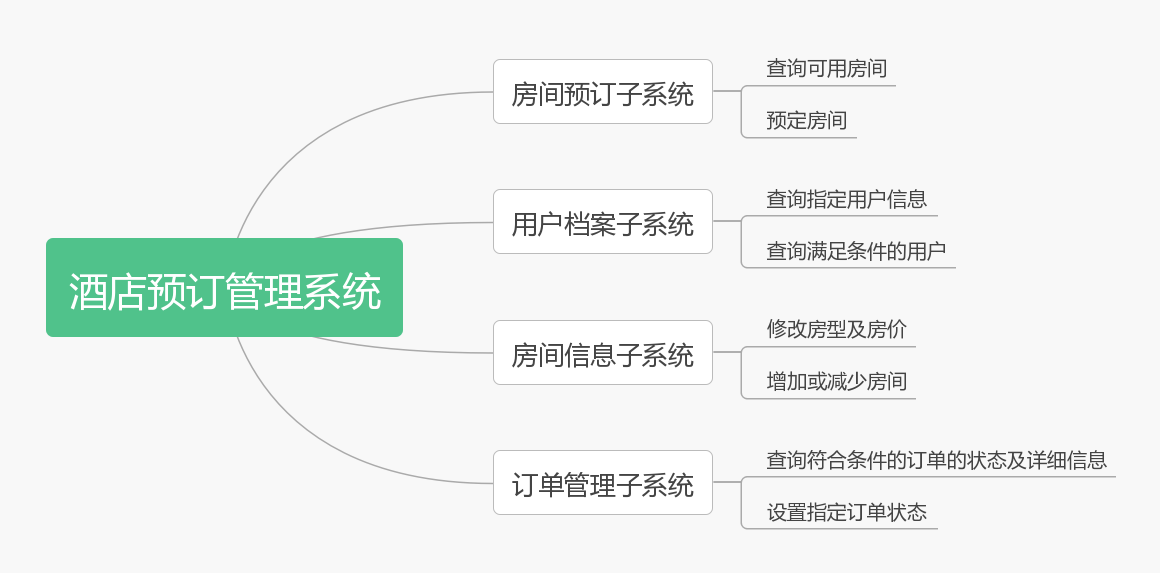
\includegraphics[width=15cm]{figure/2018-12-15-19-12-55.png}
    \caption{子系统设计}
    \label{fig:sub-system-design}
    %\end{adjustwidth}
\end{figure}


\chapter{数据库设计}
在本节中,我们会按照概念设计、逻辑设计到物理设计的顺序讲解本项目的具体设计方式。
\section{概念设计}
概念设计包括数据库的实体集、联系集和ER图。
\subsection{实体集}
描述酒店的房间需要房间实体集(\autoref{tab:E-room})和房型实体集(\autoref{tab:E-type})。
房型是指房间的
\begin{table}[htp]
    \caption{房间实体集}
    \centering
    \rowcolors{1}{White}{Lavender}
    \begin{tabular}{cccp{11cm}<{\centering}}
    \toprule
        \emph{属性}  & \emph{备注} \\
    \midrule
        \underline{id}  & 唯一 \\
        floor & 层数\\
        room\_num  & 不包括floor的房间号 \\
        price &  \\
    \bottomrule
    \hiderowcolors
    \end{tabular}
    \label{tab:E-room}
\end{table}

\begin{table}[htp]
    \caption{房型实体集}
    \centering
    \rowcolors{1}{White}{Lavender}
    \begin{tabular}{cccp{11cm}<{\centering}}
    \toprule
        \emph{属性}  & \emph{备注} \\
    \midrule
        \underline{id} & 唯一 \\
        breakfast  & 是否包含早餐 \\
        wifi & 是否包含无线网络 \\
    \bottomrule
    \hiderowcolors
    \end{tabular}
    \label{tab:E-type}
\end{table} 


\begin{table}[htp]
    \caption{用户实体集}
    \centering
    \rowcolors{1}{White}{Lavender}
    \begin{tabular}{cccp{11cm}<{\centering}}
    \toprule
        \emph{属性}  & \emph{备注} \\
    \midrule
        \underline{id}  & 唯一 \\
        region & 顾客来自的地区 \\
        credential & 证件号,唯一 \\
        name & 姓名 \\
        gender & 性别 \\
        birthdate & 出生日期 \\
        phone & 电话号码 \\
        balance & 余额 \\
    \bottomrule
    \hiderowcolors
    \end{tabular}
    \label{tab:E-user}
\end{table}

\begin{table}[htp]
    \caption{订单时实体集}
    \centering
    \rowcolors{1}{White}{Lavender}
    \begin{tabular}{cccp{11cm}<{\centering}}
    \toprule
        \emph{属性} & \emph{备注} \\
    \midrule
        id & 唯一 \\
        status & 订单状态(取消、正常)\\
        check\_in & 预订的入住时间 \\
        check\_out & 预订的最后一天\\
        
    \bottomrule
    \hiderowcolors
    \end{tabular}
    \label{tab:E-order}
\end{table}

\begin{table}[htp]
    \caption{操作明细实体集}
    \centering
    \rowcolors{1}{White}{Lavender}
    \begin{tabular}{cccp{11cm}<{\centering}}
    \toprule
        \emph{属性} & \emph{备注} \\
    \midrule
        id & 唯一 \\
        time & 操作的发生时间 \\
        detail& 操作类型(发起订单、取消订单)\\
        
    \bottomrule
    \hiderowcolors
    \end{tabular}
    \label{tab:E-operation}
\end{table}



\subsection{联系集}
\subsection{E-R图}

\section{逻辑设计}

在完成数据库的概念设计后,接下来要做的是将所有实体集合联系集分别转换为关系模式$R$。

有关实体集的转换规则如下:

\begin{itemize}
	\item 具有$n$个简单描述性属性的强实体集转换为具有$n$个属性的关系模式
	\item 为复合属性的每个子属性在$R$中创建一个单独的属性
	\item 为多值属性$M$创建一个单独的关系模式,该模式中包含了$M$所在的实体集或联系集的主码
	\item 将派生属性实现为方法
	\item 将弱实体集表示为包含所有弱实体集属性以及所依赖的强实体集的主码的关系模式。$R$的主码包括弱实体集的部分码和所以来的强实体集的主码。
\end{itemize}

有关联系集的转换规则如下:

\begin{itemize}
	\item 联系集转换为由联系集的描述性属性以及相关实体集的主码组成的关系模式
	\item 对于多对多的联系集,$R$的主码包含所有相关实体集的主码
	\item 对于一对一的联系集,任意一个相关实体集的主码都可以作为$R$的主码
	\item 对于一对多的联系集,用关联的映射基数为"多"的那个实体集作为$R$的主码
\end{itemize}

转换完成后,还要消除关系模式的冗余,并合并部分关系模式。具体而言包括以下两种情况:

\begin{itemize}
	\item 连接弱实体集与其依赖的强实体集的联系集的模式是多对一且没有描述性属性的,另外弱实体集的主码包含强实体集的主码,因此这样的联系集对应的关系模式是冗余的。
	\item 考虑多对一的联系集$AB$和相关的实体集$A$, $B$, ,若$A$在联系中的参与是全部的,那么可以将$A$与$AB$模式属性合并得到$A^*$,主码是$A$的主码,外码加入$A^*$中。
\end{itemize}

依照上述规则,由于Type、Room、Operation、Order、User、Region均为简单强实体集于是可以首先生成包含对应属性的关系模式。再考虑联系集,由于OrderUser、RoomType、OrderRoom、OrderOp、UserRegion均为一对多的联系集,因此均可以按照上述规则消除。

最后得到以下关系模式:

RoomType(\textbf{id}, breakfast, wifi)

Room(\textbf{id}, floor, room\_num, price, \textit{type\_id})

Operation(\textbf{id}, time, operation. \textit{order\_id})

Order(\textbf{id}, time, status, check\_in, check\_out, \textit{room\_id}, \textit{user\_id})

Region(\textbf{id}, name)

User(\textbf{id}, credential, name, gender, birthdate, phone, balance, \textit{region\_id})


\section{物理设计}

\chapter{数据库创建和数据加载}

TODO:要建一些view方便查询

\chapter{数据库应用软件设计与开发}


%%%%%%%%%%%%%%%%%%%%%%%%%%%%%%%%%%%%%%%%%%%%%%%%%%%%%%%%%%%%%%%%%%%%%%%%%%%%
% 参考文献
%%%%%%%%%%%%%%%%%%%%%%%%%%%%%%%%%%%%%%%%%%%%%%%%%%%%%%%%%%%%%%%%%%%%%%%%%%%%
% \cleardoublepage\phantomsection
% \addcontentsline{toc}{chapter}{参考文献}

% \bibliography{opsystem}
% \bibliographystyle{unsrt}

% \begin{thebibliography}{00}
%   \bibitem{r1} 作者. 文章题目 [J].  期刊名, 出版年份,卷号(期数): 起止页码.
%   \bibitem{r2} 作者. 书名 [M]. 版次. 出版地:出版单位,出版年份:起止页码.
%   \bibitem{r3} 邓建松等, 《\LaTeXe~科技排版指南》, 科学出版社.
%   \bibitem{r4} 吴凌云, 《CTeX~FAQ (常见问题集)》, \textit{Version~0.4}, June 21, 2004.
%   \bibitem{r5} Herbert Vo\ss, Mathmode, \url{http://www.tex.ac.uk/ctan/info/math/voss/mathmode/Mathmode.pdf}.
% \end{thebibliography}
%%%%%%%%%%%%%%%%%%%%%%%%%%%%%%%%%%%%%%%%%%%%%%%%%%%%%%%%%%%%%%%%%%%%%%%%%%%%
% 附录
%%%%%%%%%%%%%%%%%%%%%%%%%%%%%%%%%%%%%%%%%%%%%%%%%%%%%%%%%%%%%%%%%%%%%%%%%%%%
\appendix


\cleardoublepage
\end{document}